%%% Choose between 16:9 and 4:3 format by commenting out/uncommenting one of the following lines:
\documentclass[aspectratio=169]{beamer} % 16:9
% \documentclass{beamer} % 4:3

%=========================================================================================================================

\usepackage[english]{babel}     % English language
\usepackage[utf8]{inputenc}     % Input encoding changed to utf8 for proper rendering of umlauts
\usepackage{tikz}               % For creating graphics
\usepackage{subfig}
\usepackage[mode=buildnew]{standalone}
\usepackage{url}                % For including urls
\usepackage{tabularx}           % For better tables
\usepackage{xcolor}             % Für bunte Farbe :)

\usetheme{aig}                  % Set beamer theme


%%% commands
\newcommand{\clf}{\operatorname{clf}}
\newcommand{\rec}{\operatorname{rec}}
\newcommand{\tp}{\operatorname{TP}}
\newcommand{\tn}{\operatorname{TN}}
\newcommand{\fp}{\operatorname{FP}}
\newcommand{\fn}{\operatorname{FN}}

%=========================================================================================================================
\title{Qualität von Wikipedia-Artikeln}
\author[Kunze, Bunge, Krämer, Steenhof, Suxdorf]{Alexander Kunze, Sebastian Bunge, Johannes Krämer, Emmanuelle Steenhof, Robin Suxdorf}
\institute{Artificial Intelligence Group,\\
University of Hagen, Germany}
\date{\today}
%=========================================================================================================================
\logo{
\includegraphics[width=3cm]{figures/logoaig.png}}
%=========================================================================================================================

\begin{document}

%=========================================================================================================================

% frame
% block
% alertblock
% exampleblock

% \highlight{}
% \darkhighlight{}
% \yellowhighlight{}
% \mathhighlight{}
% \darkmathhighlight{}
% \yellowmathhighlight{}

% appendix

\begin{frame}
    \titlepage
\end{frame}
\nologo

\begin{frame}{Motivation}
    \begin{figure}
        \centering
        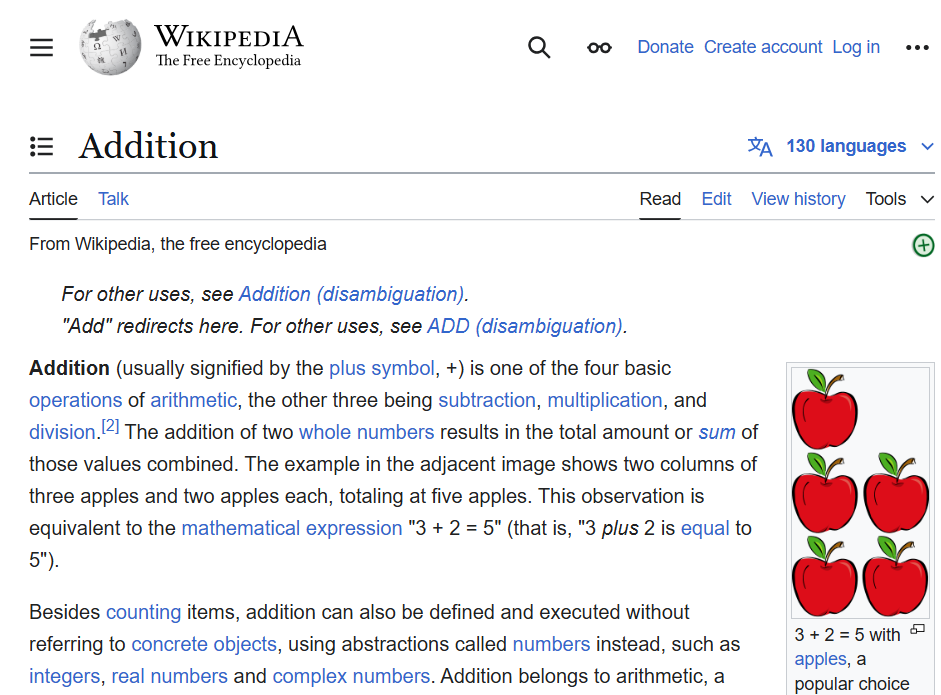
\includegraphics[width=0.6\linewidth]{figures/wp-screenshot-good.png}
        \caption{\url{https://en.wikipedia.org/wiki/Addition}}
    \end{figure}
\end{frame}

\begin{frame}{Motivation}
    \begin{figure}
        \centering
        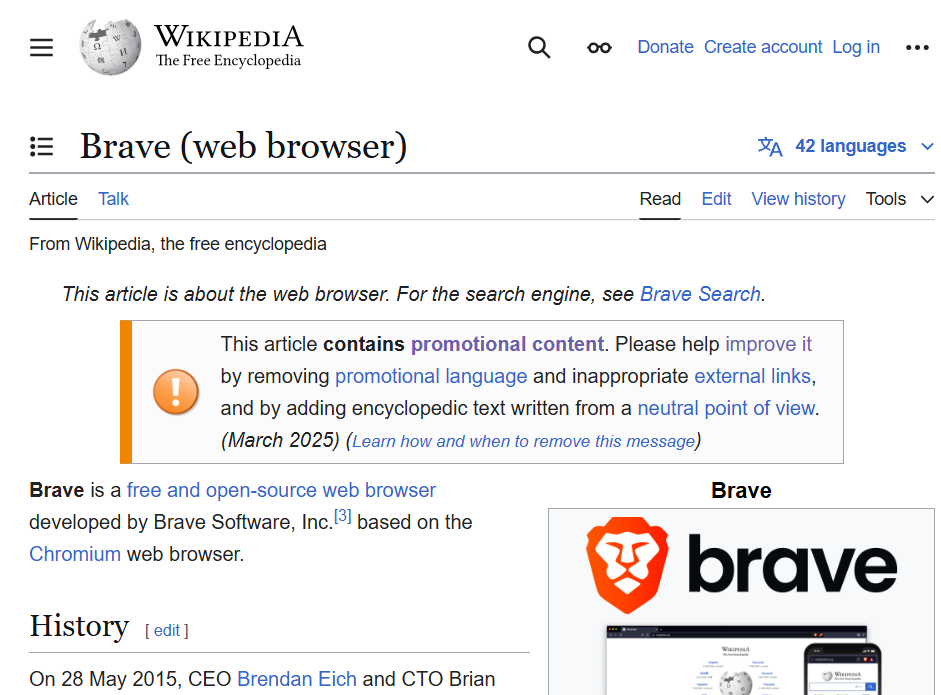
\includegraphics[width=0.6\linewidth]{figures/wp-screenshot-promo.png}
        \caption{\url{https://en.wikipedia.org/wiki/Brave_(web_browser)}}
    \end{figure}
\end{frame}

\begin{frame}{Motivation}
    \begin{figure}
        \centering
        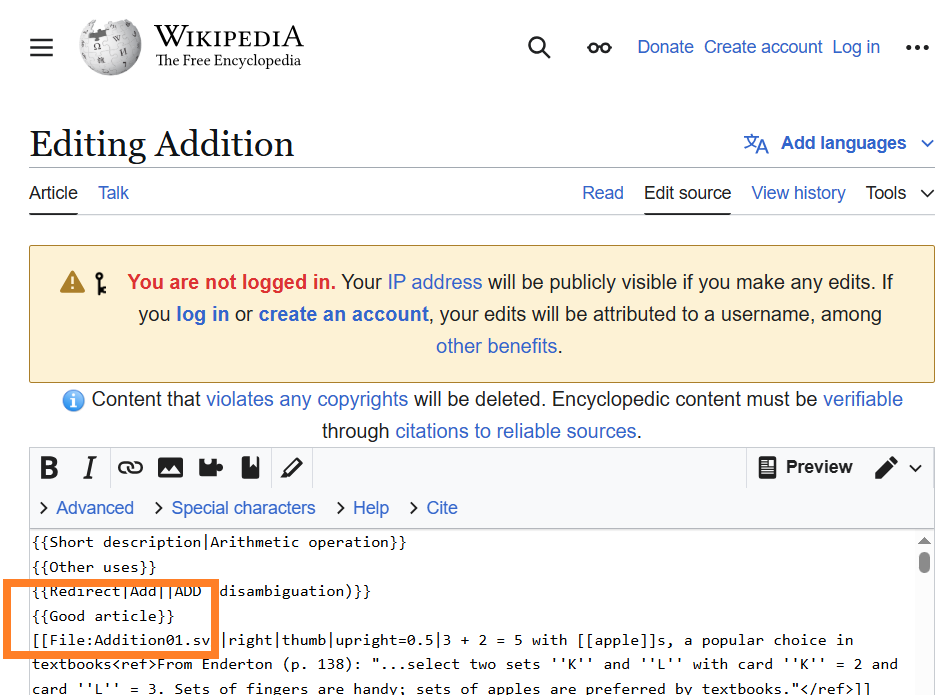
\includegraphics[width=0.6\linewidth]{figures/wp-screenshot-good-source.png}
        \caption{\url{https://en.wikipedia.org/w/index.php?title=Addition&action=edit}}
    \end{figure}
\end{frame}

\begin{frame}{Motivation}
    \begin{figure}
        \centering
        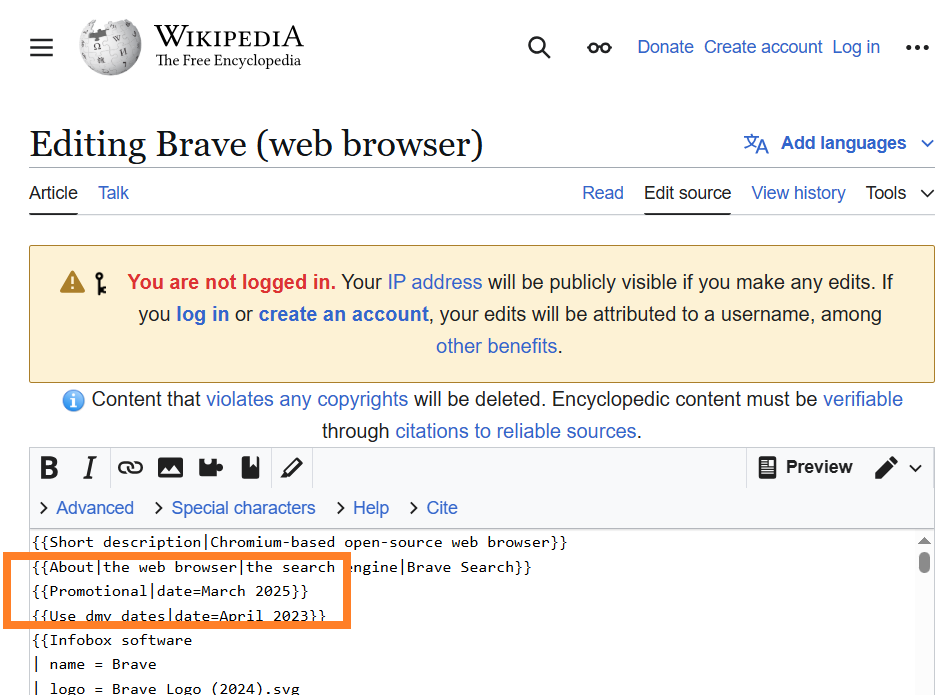
\includegraphics[width=0.6\linewidth]{figures/wp-screenshot-promo-source.png}
        \caption{\url{https://en.wikipedia.org/w/index.php?title=Brave_(web_browser)&action=edit}}
    \end{figure}
\end{frame}

\begin{frame}{Overview}
\tableofcontents
\end{frame}

\section{Daten}

\subsection{Problemstellung}

\begin{frame}{Problemstellung}
    \begin{block}{Good articles}
        \begin{itemize}
            \item Müssen unter anderem die folgenden Kriterien erfüllen:
                  \begin{itemize}
                      \item gut geschrieben
                      \item korrekte und überprüfbare Informationen
                      \item neutral in der Sichtweise
                      \item verwenden relevante Bilder mit geeigneten Urheberrechtslizenzen
                  \end{itemize}
            \item Nominierung und Vergabe des Status durch die Community (Good article nomination).
            \item 0.59\% aller Wikipedia-Artikel
        \end{itemize}
    \end{block}
\end{frame}

\begin{frame}{Problemstellung}
    \begin{block}{Articles with a promotional tone}
        \begin{itemize}
            \item Artikel, die aus folgenden Gründen einer Überarbeitung bedürfen:
                  \begin{itemize}
                      \item Werbung
                      \item Interessenkonflikte
                      \item Aus Sicht eines Fans
                      \item Pressemitteilungen
                      \item Wie ein Lebenslauf
                  \end{itemize}
            \item Entsprechende Templates können durch jeden Autoren zum Artikel hinzugefügt oder entfernt werden.
        \end{itemize}
    \end{block}
\end{frame}

\begin{frame}{Problemstellung}
    \begin{block}{Problemstellung}
        \begin{itemize}
            \item \textbf{Binäre Klassifikation}: Gehört ein gegebener Artikel zu den guten Artikeln oder hat er einen werbenden Ton?
            \item \textbf{Multiclass-Klassifikation}: Gehört er alternativ zu der großen Klasse der Artikel, die weder besonders gut sind, noch einen werbenden Ton haben?
            \item \textbf{Multilabel-Klassifikation}: Aus welchen Gründen hat ein Artikel einen werbenden Ton?
        \end{itemize}
    \end{block}
\end{frame}

\subsection{Datensatz}

\begin{frame}{Datensatz}
    \begin{block}{Kaggle - Wikipedia Promotional Articles}
        \begin{itemize}
            \item Hochgeladen Oktober 2019.
            \item Enthält alle Artikel der englischen Wikipedia, die zum damaligen Zeitpunkt als "good" bzw. "with a promotional tone" markiert waren.
            \item Aufgeteilt auf zwei CSV-Dateien: \texttt{good.csv}, \texttt{promotional.csv}.
            \item \texttt{good.csv} enthält die Spalten \texttt{text} und \texttt{url}.
            \item \texttt{promotional.csv} enthält außerdem für jedes mögliche Label eine Spalte: \texttt{advert}, \texttt{coi}, \texttt{fanpov}, \texttt{pr}, \texttt{resume}
        \end{itemize}
    \end{block}
\end{frame}

\begin{frame}{Datensatz}
    \begin{figure}
        \centering
        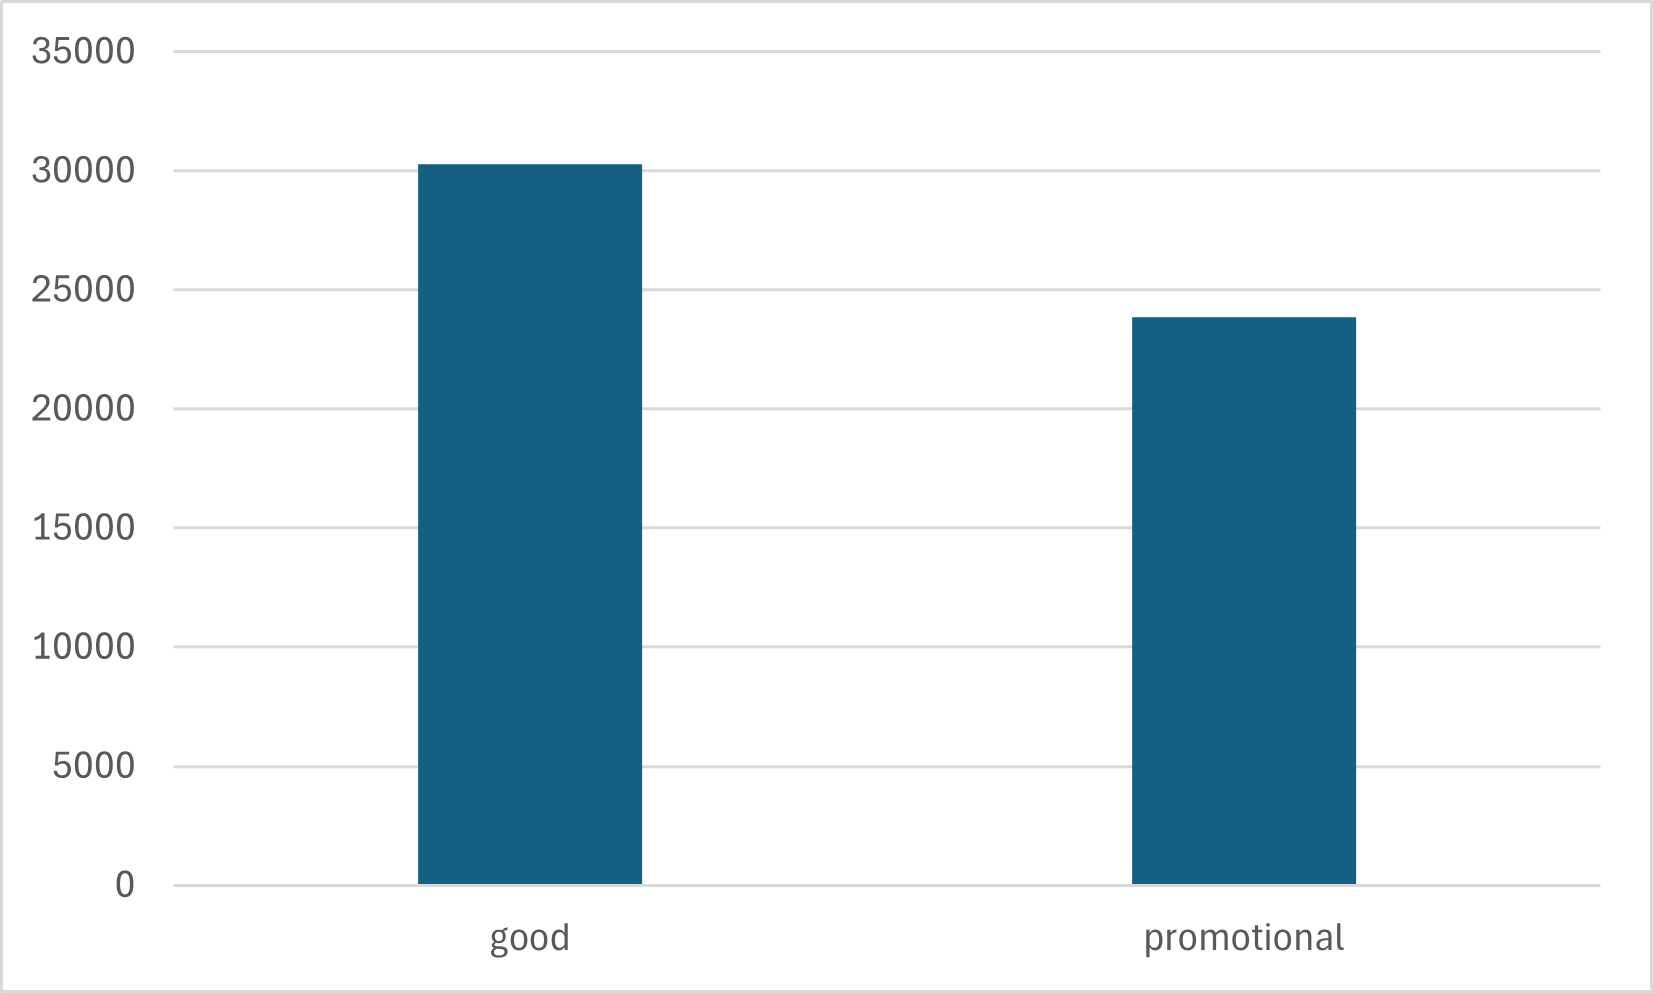
\includegraphics[width=0.6\linewidth]{figures/kaggle-classes.png}
        \caption{Kaggle - Wikipedia Promotional Articles (Classes)}
    \end{figure}
\end{frame}

\begin{frame}{Datensatz}
    \begin{figure}
        \centering
        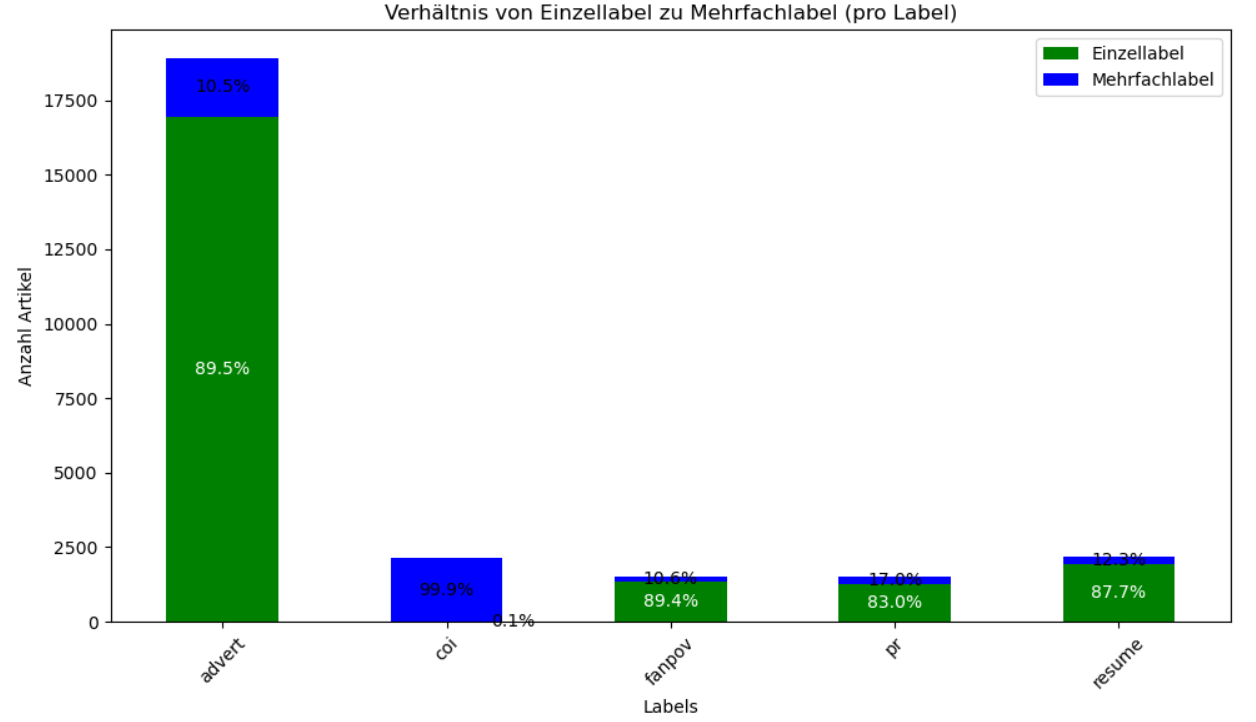
\includegraphics[width=0.6\linewidth]{figures/kaggle-promo-labels-2.png}
        \caption{Kaggle - Wikipedia Promotional Articles (Labels)}
    \end{figure}
\end{frame}

\subsection{Weitere Daten}

\begin{frame}{Weitere Daten}
    \begin{block}{Einschränkungen des Kaggle-Datensatzes}
        \begin{itemize}
            \item Nicht mehr aktuell: Stand 2019.
            \item Fast 99\% der Artikel sind nicht enthalten, weil sie zu keiner der beiden Klassen gehören.
        \end{itemize}
    \end{block}
\end{frame}

\begin{frame}{Weitere Daten}
    \begin{block}{Wikipedia-Dump}
        \begin{itemize}
            \item Abzüge aller Wikimedia-Datenbanken werden zum Download angeboten.
            \item Aktualisierung zwei Mal monatlich (Angaben beziehen sich auf Dez. 2024).
            \item Englischsprachige Wikipedia ohne Historie ca. 22 GB komprimiert, 97 GB entpackt.
            \item Enthält ca. 24 Mio. Wikipedia-Seiten, darunter ca. 7 Mio. Artikel.
            \item Konvertierung:
                  \begin{itemize}
                      \item Entpacken und Verarbeiten in Blöcken von je 100 Seiten.
                      \item Nicht-Artikel-Seiten erkennen und ausschließen.
                      \item Erkennen der Klassen und Label anhand von Templates im Quelltext.
                  \end{itemize}
        \end{itemize}
    \end{block}
\end{frame}

\begin{frame}{Weitere Daten}
    \begin{block}{Wikipedia-Dump - Verteilung}
        %\begin{table}
        %    \centering
        %    \begin{tabular}{cc}
        %        good & 46.882 \\
        %        promotional & 32.633 \\
        %        neutral & 6.611.303 \\
        %    \end{tabular}
        %\end{table}
        \begin{itemize}
            \item Klassen der englischsprachigen Artikel:
                  \begin{itemize}
                      \item good: 46.882
                      \item promotional: 32.633
                      \item neutral: 6.611.303
                  \end{itemize}
            \item Stark unausgeglichen, Reduktion durch Undersampling.
        \end{itemize}
    \end{block}
\end{frame}

\subsection{Vorverarbeitung}

\begin{frame}{Vorverarbeitung}
    \begin{block}{Datensatzvorverarbeitung}
        \begin{itemize}
            \item Extrahieren von Labeln aus Metadaten
            \item Reduzieren auf Artikeltext und Label
            \item Zusammenführen mehrerer Dateien in ein DataFrame
        \end{itemize}
    \end{block}
    \begin{block}{Textvorverarbeitung}
        \begin{itemize}
            \item Entfernen von Sonder- und Interpunktionszeichen
            \item Umwandeln in Kleinbuchstaben
            \item Entfernen von Stoppwörtern
            \item Umwandeln mit Stemming (PorterStemmer)
            \item Zahlen bleiben erhalten
        \end{itemize}
    \end{block}
\end{frame}

% Kandidat für Appendix
\begin{frame}{Vorverarbeitung}
    \begin{exampleblock}{Textvorverarbeitung Artikel 39582}
        \begin{tabularx}{\textwidth}{>{\raggedright\arraybackslash}X >{\raggedright\arraybackslash}X}
            \textbf{Original} & \textbf{Verarbeitete Version}                                                                                                                                                                                                 \\ \hline
            The Human Research Program HRP was created in October 2005 at Johnson Space Center JSC in response to NASA's desire to move human research project management away from headquarters to JSC and to focus its research investment on investigating and mitigating the highest risks to astronaut health and performance in support of exploration missions...
                              &
            human research program hrp creat octob 2005 johnson space center jsc respons nasa desir move human research project manag away headquart jsc focu research invest investig mitig highest risk astronaut health perform support explor mission ... \\
        \end{tabularx}
    \end{exampleblock}
\end{frame}

\begin{frame}{Vorverarbeitung}
    \begin{block}{TF-IDF Vektorisierung}
        \begin{itemize}
            \item Term Frequency-Inverse Document Frequency (TF-IDF) zur Textvektorisierung
            \item Bewertet Wichtigkeit eines Wortes in einem Dokument relativ zum Korpus
            \item Vorteile:
                  \begin{itemize}
                      \item Reduziert Einfluss häufiger, aber uninformativer Wörter
                      \item Hebt diskriminierende Begriffe hervor
                      \item Erzeugt spärliche Merkmalsvektormatrizen
                  \end{itemize}
            \item Parameter:
                  \begin{itemize}
                      \item \texttt{ngram\_range: [1, 1]} - Nur Einzelwörter werden betrachtet
                            % Mehrwort-Ausdrücke (n-grams) werden nicht berücksichtigt
                      \item \texttt{max\_df: 0.9} - Ignoriert Korpus-spezifische Stopwörter ($>90\%$)
                            % Entfernt häufige Wörter, die in fast allen Dokumenten vorkommen
                      \item \texttt{min\_df: 0.001} - Filtert Rauschen und Rechtschreibfehler ($<0.1\%$)
                            % Entfernt sehr seltene Wörter, reduziert Vokabulargröße und Overfit-Risiko
                      \item \texttt{max\_features: 10\_000} - Beschränkt die Vokabulargröße auf 10.000
                            % Verbessert Laufzeiteffizienz und verringert Overfit-Risiko
                      \item \texttt{sublinear\_tf: true} - Logarithmische TF-Skalierung für lange Dokumente
                            % Reduziert Verzerrungen durch mehrfach vorkommende Wörter in einem Dokument
                  \end{itemize}
        \end{itemize}
    \end{block}
\end{frame}

\begin{frame}{Easy Data Augmentation (EDA)}
    \begin{block}{Ziel und Methode}
        \begin{itemize}
            \item Idee: Die Anwendung von Easy Data Augmentation (EDA), um durch augmentierte Daten die Anzahl der unterrepräsentierten Labels zu vergrößern.
        \end{itemize}
    \end{block}

    \begin{block}{Umsetzung}
        \begin{itemize}
            \item Es wurden neue Texte aus den Originaltexten erstellt indem Synonyme hinzugefügt, zufällig Wortreihenfolgen getauscht und zufällig Wörter eingefügt bzw. gelöscht worden sind.
        \end{itemize}
    \end{block}

    \begin{block}{Ergebnisse}
        \begin{itemize}
            \item Das Modell war signifikant besser, wenn auf den augmentierten Daten getestet worden ist, schnitt bei Tests auf dem Originalsatz aber deutlich schlechter ab. Damit zeigt sich der Verdacht von Overfitting. $\to$ \textbf{Ansatz verworfen}.
        \end{itemize}
    \end{block}
\end{frame}

\section{Ansätze}

\begin{frame}{Ansätze}
    \begin{block}{Klassische Verfahren}
        \begin{itemize}
            \item Logistische Regression
            \item Bayes-Klassifikator
            \item Support Vector Machine
        \end{itemize}
    \end{block}
    \begin{block}{Deep Learning}
        \begin{itemize}
            \item Künstliches Neuronales Netz
            \item Transformer-Ansatz
        \end{itemize}
    \end{block}
\end{frame}

\subsection{Klassische Verfahren}

\begin{frame}{Klassische Verfahren}
    \begin{block}{Logistische Regression}
        \begin{itemize}
            \item Binärer Klassifikator, der Wahrscheinlichkeiten für Klassen berechnet und eine Entscheidungsgrenze anhand eines Schwellenwerts setzt.
            \item Vorteile:
                  \begin{itemize}
                      \item Einfach zu implementieren.
                      \item Schnell in der Berechnung.
                  \end{itemize}
                  %\item Parameter:
                  %      \begin{itemize}
                  %          \item \texttt{Regularisierung}: L1-Regularisierung und L2-Regularisierung
                  % Wird verwendet, um Überanpassung zu vermeiden, indem große Koeffizienten bestraft werden
                  %          \item \texttt{Solver}: \texttt{liblinear} und \texttt{saga}
                  % liblinear ist der Standardsolver, saga ist besonders geeignet für große Datenmengen
                  %      \end{itemize}
        \end{itemize}
    \end{block}
\end{frame}

\begin{frame}{Klassische Verfahren}
    \begin{block}{Multinomialer Naive Bayes-Klassifikator}
        \begin{itemize}
            \item Probabilistischer Klassifikator, der auf dem Bayes-Theorem basiert.
            \item Nimmt bedingte Unabhängigkeit zwischen Features an (naive Annahme).
            \item Geeignet für Textklassifikation mit Wortvorkommen als Features.
            \item Vorteile:
                  \begin{itemize}
                      \item Lineare Zeitkomplexität O(nd) % n = Anzahl der Features, d = Anzahl der Samples
                            % Mit Abstand der schnelleste Klassifikator gerade beim gesampelten Wikipedia-Dump
                            % Training auf den Dump-Samples war nach Sekunden abgeschlossen
                      \item Robust bei hoher Dimensionalität
                            % Die vektorisierten Features sind hochdimensional
                      \item Native Unterstützung für spärliche Matrizen
                            % die vektorisierten Features sind spärliche Matrizen
                  \end{itemize}
                  %\item Parameter:
                  %      \begin{itemize}
                  %          \item \texttt{alpha}: Laplace-Glättung
                  % Wird verwendet, um Überanpassung zu vermeiden, indem Null-Wahrscheinlichkeiten durch eine kleine positive Konstante ersetzt werden
                  %          \item \texttt{fit\_prior}: Lernen der Klassenpriors
                  % Wird verwendet, um die Klassenverteilung aus den Trainingsdaten zu schätzen bevor man irgendwelche Features sieht. Wenn False wird gleiche Klassenwahrscheinlichkeit angenommen
                  %      \end{itemize}
        \end{itemize}
    \end{block}
\end{frame}

\begin{frame}{Klassische Verfahren}
    \begin{block}{Support Vector Machine (SVM)}
        \begin{itemize}
            \item Nutzt das Konzept des maximalen Margins, um eine möglichst gut trennende Hyperebene zu finden.
            \item Erweiterbar durch Kernelfunktionen für nicht-lineare Trennungen.
            \item Leistungsfähig für hoch-dimensionale Daten, z.B. Textklassifikation, jedoch rechenintensiv bei großen Datensätzen
                  %\item Parameter:
                  %      \begin{itemize}
                  %          \item \texttt{C}: Regularisierungsparameter zur Steuerung des Trade-offs zwischen Maximierung des Margins und Minimierung von Fehlklassifikationen
                  %          \item \texttt{kernel}: Auswahl der Kernel-Funktion (z.B. linear, RBF, polynomial, sigmoid)
                  %          \item Kernel-spezifische Parameter (z.B. \texttt{degree} für polynomiale Kernel)
                  %      \end{itemize}
        \end{itemize}
    \end{block}
\end{frame}


\begin{frame}
    \begin{block}{Gemeinsamkeiten}
        \begin{itemize}
            \item \texttt{GridSearchCV} von Scikit-Learn wurde für eine Hyperparameter-Optimierung verwendet
            \item \texttt{OneVsRestClassifier} von Scikit-Learn wurde für Multilabel-Klassifikation verwendet
        \end{itemize}
    \end{block}
\end{frame}

\subsection{Deep Learning}

\begin{frame}{Deep-Learning}
    \begin{block}{Neuronales Netzwerk zur Klassifikation von Wikipedia-Artikeln}
        \begin{itemize}
            \item Mehrschichtiges Perzeptron (MLP) mit zwei voll verbundenen Schichten:
                  \begin{itemize}
                      \item Eingabeschicht: 10000 Features durch TF-IDF
                      \item Verborgene Schicht: 512 Neuronen, ReLU-Aktivierung
                      \item Ausgabeschicht:
                            \begin{itemize}
                                \item 2 Neuronen (binäre Klassifikation)
                                \item 3 Neuronen (multiclass Klassifikation)
                                \item 5 Neuronen (multilabel Klassifikation)
                            \end{itemize}
                  \end{itemize}
            \item Dropout (50\%) zur Regularisierung
            \item Verlustfunktion: Cross Entropy
                  \begin{equation*}
                      \mathcal{L} = - \sum_{i=1}^{C} y_i \log(\hat{y}_i)
                  \end{equation*}
        \end{itemize}
    \end{block}
\end{frame}

\begin{frame}{Deep Learning}
    \begin{block}{5. Ansatz}
        \begin{itemize}
            \item Probleme: Schlechte Multilabelklassifizierung der ersten vier Ansätze.
            \item    Analyse: Unterscheidung der Promotional aufgrund von Thema
            \item        Ziel:
                  Einbezug von Kontext/Bedeutung \\
            \item Ideen:
                  \begin{itemize}
                      \item Vorverarbeitungsmethode erstellen
                      \item Transformerarchitektur verwenden
                  \end{itemize}
        \end{itemize}
    \end{block}
\end{frame}

\begin{frame}{Deep Learning}
    %\begin{block}{Arbeitsweise von Transformern}
    \begin{center}
        \begin{figure}
            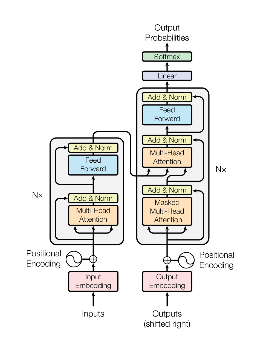
\includegraphics[scale=1.2]{figures/TransformerArchitektur.eps}
            \caption{Architektur Transformer}
        \end{figure}
    \end{center}
    %\end{block}
\end{frame}


\begin{frame}{Deep Learning}
    %\begin{block}{Arbeitsweise von Transformern}
    \begin{center}
        \begin{figure}
            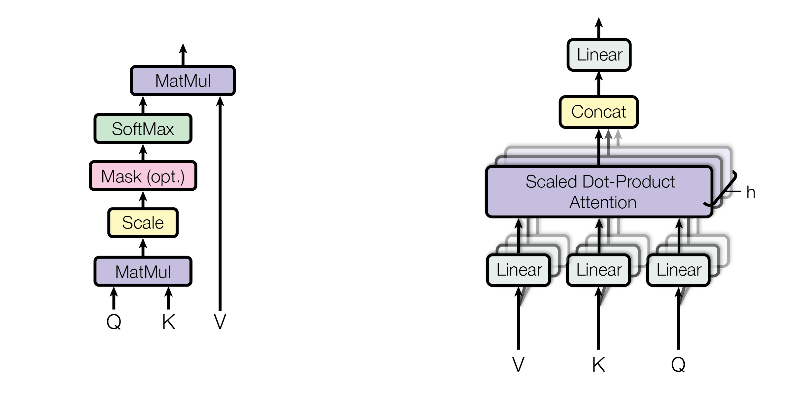
\includegraphics[scale=0.9]{figures/TransformerAttention.eps}
            \caption{Transformer Attention; Links: Scaled dot product attention; Rechts: Multi-head-Attention}
        \end{figure}
    \end{center}
    %\end{block}
\end{frame}



\begin{frame}{Deep Learning}
    \begin{block}{Bidirectional Transformers for Language Understanding (BERT)}
        \begin{itemize}
            \item Vorteil: Besondere Fähigkeit zur Erkennung von Kontext
            \item Transfer Learning:
                  \begin{itemize}
                      \item Pretraining auf ungelabelten Daten
                      \item Fine-Tuning auf gelabelten Daten
                  \end{itemize}
            \item Tokenizer: WordPiece Embeddings
            \item Attention: Bidirectional Cross-Attention
        \end{itemize}
    \end{block}
\end{frame}


\begin{frame}{Deep Learning}
    \begin{block}{Transformerarchitektur}
        \begin{itemize}
            \item Modellwahl: DistilBERT \\
            \item  Architektur:
                  \begin{itemize}
                      \item Darstellung: DistilBERT Tokenizer %Vokabular: 30522 Wörter
                      \item Encoder: 6 Schichten
                      \item Feedforwardschichten Encoder: 3072 Neuronen
                            % \item Multi-Attention-Heads: 12
                      \item Dropout: 0.2
                      \item Attention: Scaled Dot Product Attention (SDPA)
                      \item Aktivierungsfunktion: $GELU(x) = x \cdot P(X \leq x) = x \cdot \Phi(x) $
                            % \item Loss-funktion: Cross Entropy
                      \item Optimizer: AdamW
                  \end{itemize}
        \end{itemize}
    \end{block}
\end{frame}



\begin{frame}{Deep Learning}
    \begin{block}{Strukturelle Eigenschaften}
        \begin{itemize}
            \item Binäre Klassifikation:
                  \begin{itemize}
                      \item 2 Ausgabe Neuronen
                  \end{itemize}
            \item Multiklassenklassifikation
                  \begin{itemize}
                      \item 3 Ausgabe Neuronen
                      \item Cross-Attention
                  \end{itemize}
            \item Multilabel
                  \begin{itemize}
                      \item 5 Ausgabeneuronen
                      \item Cross-Attention
                      \item Advert-Ausgabeneuron versehen mit Sigmoid-Aktivierungsfunktion Schwellwert 0.5
                      \item Coi, Fanpov, PR, Resume mithile von Anomalieerkennung
                  \end{itemize}
        \end{itemize}

    \end{block}
\end{frame}



\section{Resultate}

\begin{frame}{Metriken}
    \begin{block}{Metriken}
        \begin{itemize}
            \item Binäre Klassifikation: Sei $\clf\colon \mathbb{R}^d\to \{0, 1\}$ ein binärer Klassifikator. Dann betrachten wir die  \textbf{Sensitivität(Recall)}
                  \begin{equation*}
                      \rec(D, \clf) = \frac{\tp(D, \clf)}{\tp(D, \clf) + \fn(D, \clf)}.
                  \end{equation*}

            \item Multilabel Klassifikation: Sei $\clf_i\colon\mathbb{R}^d\to\{0, 1\}$ ein binärer Klassifikator für das Label $i$. Dann betrachten wir den \textbf{macro average recall}
                  \begin{equation*}
                      \operatorname{macro\,avg\,rec}(D, \clf) = \frac{1}{k}\sum_{i=1}^k\rec (D, \clf_i).
                  \end{equation*}
        \end{itemize}
    \end{block}
\end{frame}

\begin{frame}{Resultate: Sensitivität}
    \begin{center}
        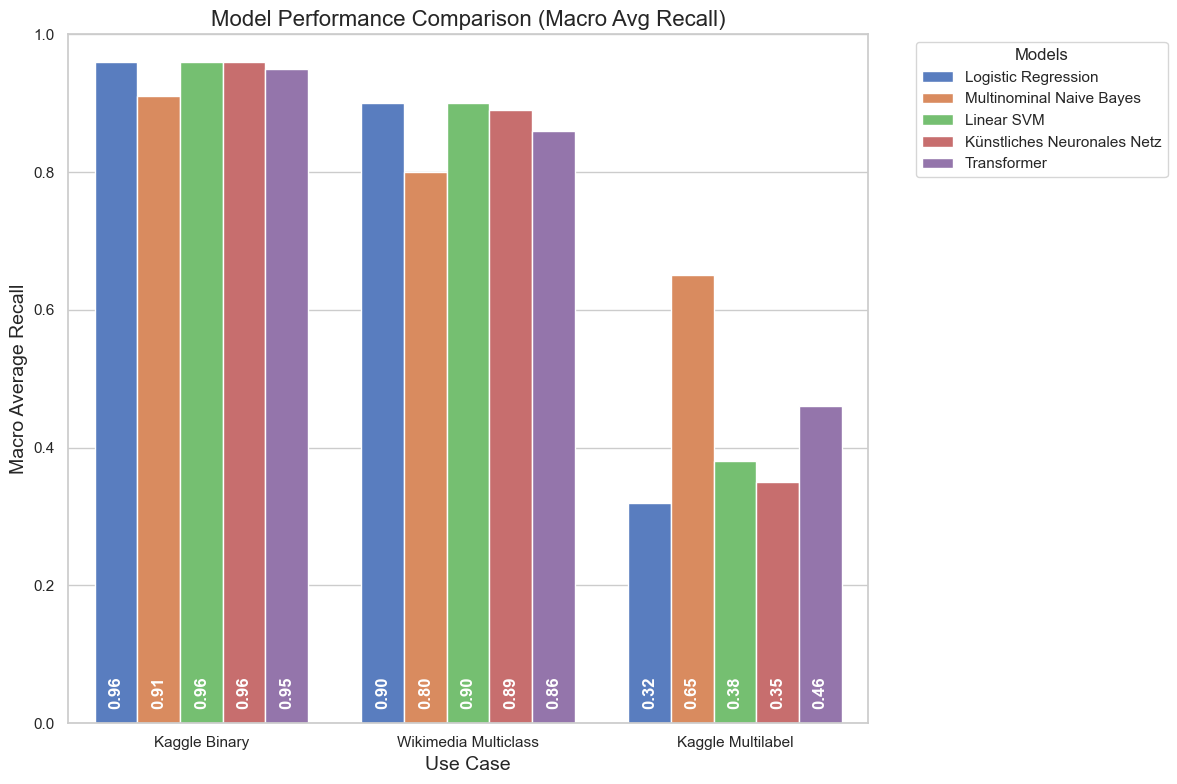
\includegraphics[scale=0.35]{figures/macro_avg_recall_usecases.png}
    \end{center}
\end{frame}

\begin{frame}{Resultate: Präzision}
    \begin{center}
        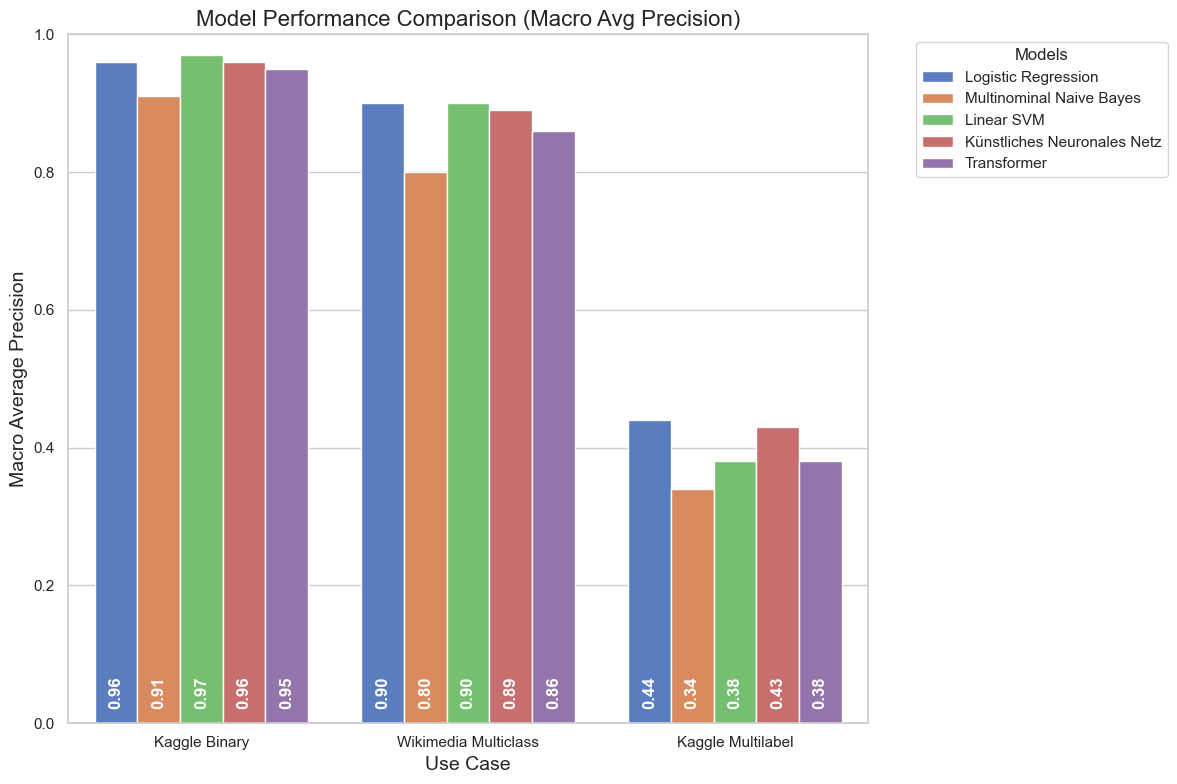
\includegraphics[scale=0.35]{figures/macro_avg_precision_usecases.png}
    \end{center}
\end{frame}

\begin{frame}{Resultate: Augmentierte Daten}
    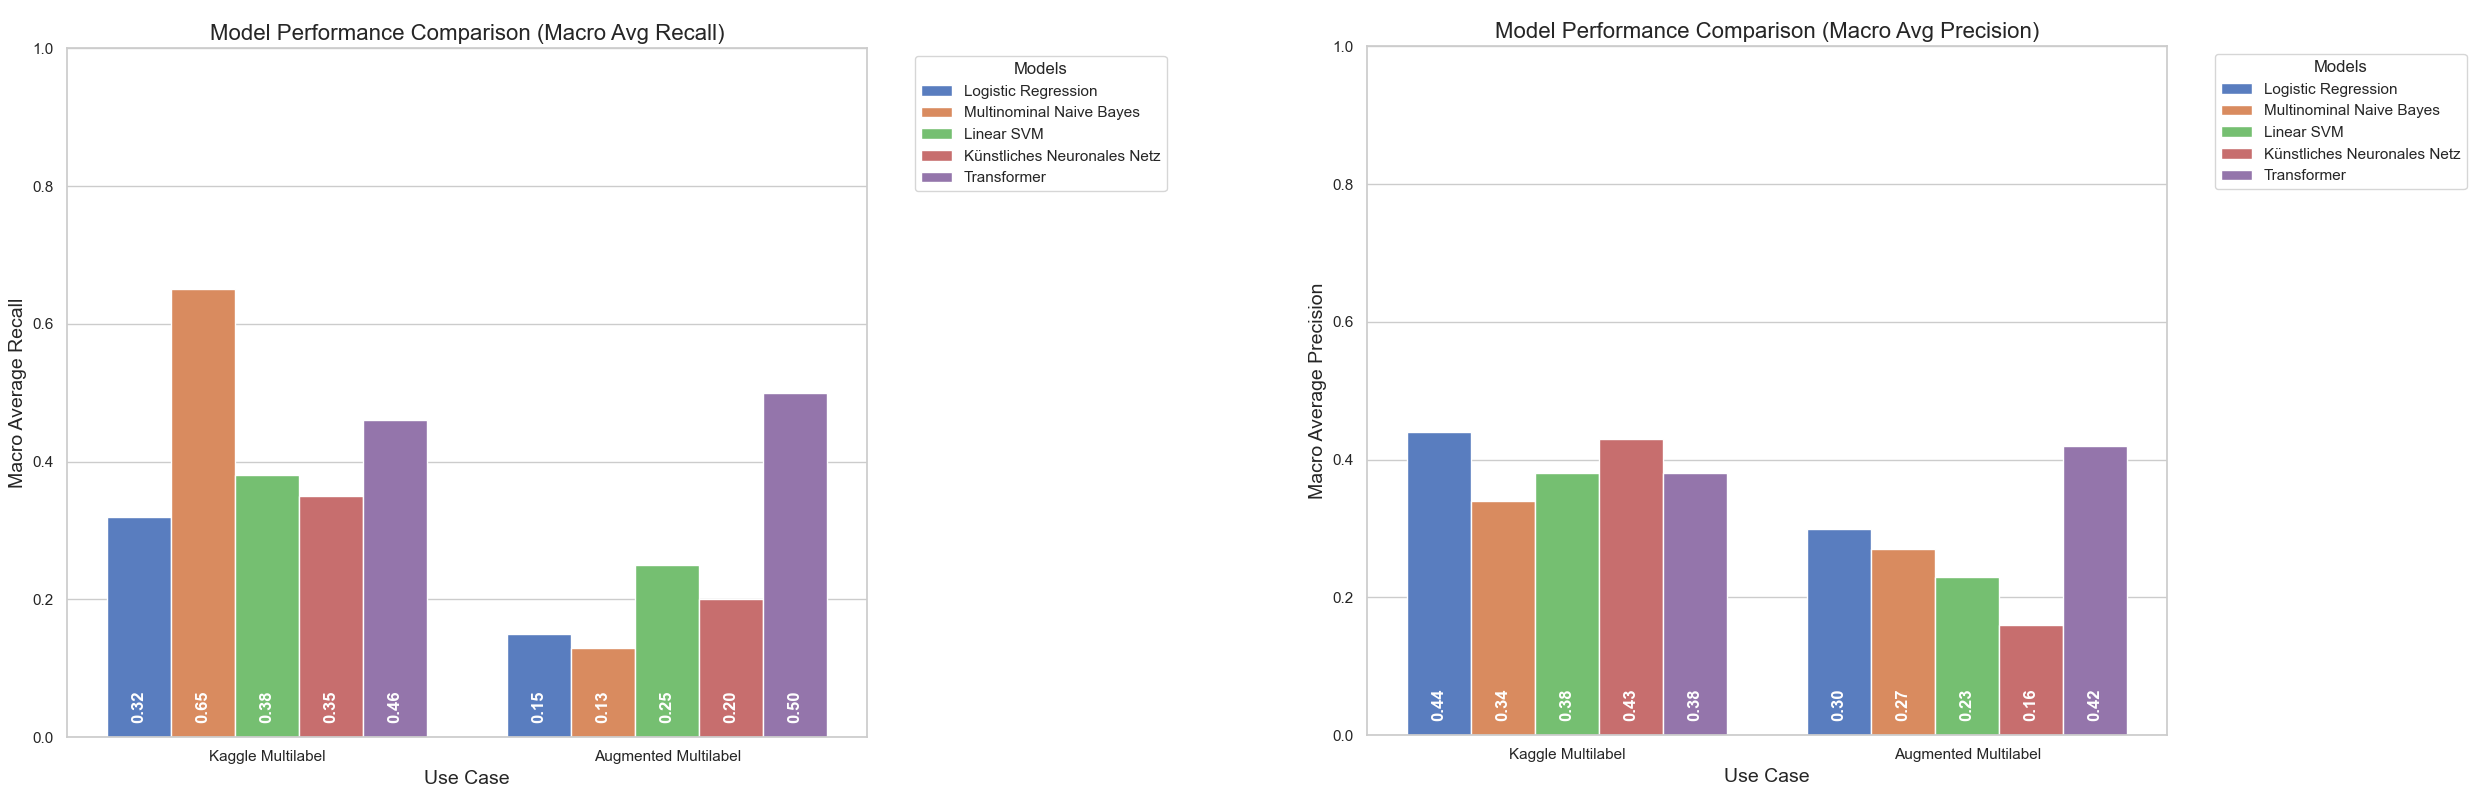
\includegraphics[scale=0.7]{figures/AugmentierteDatenVergleichZusammen.png}
\end{frame}

\begin{frame}{Resultate}
    \begin{block}{Evaluation}
        \begin{itemize}
            \item Binäre Klassifizierung
                  \begin{itemize}
                      \item Sensitivität: 96 Prozent
                      \item Beste Modelle: KNN, SVM und Logistische Regression
                  \end{itemize}
            \item Multiklassenklassifizierung
                  \begin{itemize}
                      \item Sensitivität: 90 Prozent
                      \item Beste Modelle: SVM und Logistische Regression
                  \end{itemize}
            \item Multilabel
                  \begin{itemize}
                      \item Sensitivität: 66 Prozent
                      \item Bestes Modell: Bayes
                  \end{itemize}
        \end{itemize}
    \end{block}
\end{frame}

\section{Zusammenfassung}

\begin{frame}{Zusammenfassung}
    \begin{block}{Zusammenfassung}
        \begin{itemize}
            \item Errungenschaften
                  \begin{itemize}
                      \item Daten analysiert und erweitert
                      \item Problemstellung erfasst
                      \item Datensatz für Verfahren des maschinellen Lernens vorbereitet.
                      \item Drei klassische Modelle implementiert
                      \item Zwei neuronale Methoden implementiert
                      \item Ergebnisse evaluiert
                  \end{itemize}
            \item Misserfolge
                  \begin{itemize}
                      \item Datenaugmentierung
                      \item Entwicklung von Vorverarbeitungsmethoden zur Erkennung von Kontext
                      \item Multilabelklassifikation hat noch keinen Industriestandard
                  \end{itemize}
        \end{itemize}
    \end{block}
\end{frame}

\begin{frame}{Zusammenfassung}
    \begin{block}{Zusammenfassung}
        \begin{itemize}
            \item Ergebnisse
                  \begin{itemize}
                      \item Datensatz aus Wikipedia Dump erstellt
                      \item Pipeline zur Klassifizierung von Wikipedia-Artikeln implementiert
                      \item Modelle mit sehr guten Resultaten für Binäre und Dreiklassenklassifizierung entwickelt
                  \end{itemize}
                  Erweiterungsmöglichkeiten:
                  \begin{itemize}
                      \item Weitere klassische und neuronalen Ansätze implementieren und evaluieren
                            %\item Ganzen Wikipedia Dump verwenden
                      \item Verwendung von SetFit
                      \item Nicht-Maschinelle Lernmethoden verwenden
                  \end{itemize}
        \end{itemize}
    \end{block}
    
    \begin{center}
    \textbf{Danke für Ihre Aufmerksamkeit!}
    \end{center}
    
    \nocite{hendrycks2023gaussianerrorlinearunits}
    \nocite{Sanh2019DistilBERTAD}
    \nocite{tunstall2022efficientfewshotlearningprompts}
    \nocite{9783960108535}
    \nocite{article_comparing_LLMs}
    \nocite{Attention}
    \nocite{BERTReference}
    \nocite{das2024languageagnosticmodelingwikipediaarticles}
    \nocite{DBLP:journals/corr/BojanowskiGJM16}
    \nocite{eyheramendy_2003}
    \nocite{huggingfaceQuelle}
    \nocite{maron_1961}
    \nocite{pytorchRef}
    \nocite{shavarani2020multiclassmultilingualclassificationwikipedia}
    \nocite{skicitLearnRef}
    \nocite{textCategorizationWithSVM}
    \nocite{UrsprungDatensatz}
    \nocite{yang2019zerotraining}
    \nocite{yenduri2023generativepretrainedtransformercomprehensive}
    \nocite{ReservoirSampling}
    \nocite{Ansel2024}
    \nocite{Bishop2019}
    \nocite{Bojanowski2016}
    \nocite{Das2024}
    \nocite{Devlin2018}
    \nocite{Hendrycks2016}
    \nocite{Joachims1998}
    \nocite{Manning2009}
    \nocite{Mikolov2013}
    \nocite{Pedregosa2011}
    \nocite{Pennington2014}
    \nocite{Porter2006}
\end{frame}

\bibliographystyle{plain}
\bibliography{references.bib}
\appendix
\section{Appendix}

\begin{frame}{Ergebnisse Datenaugmentierung}
    Beispielfolie für Appendix
\end{frame}


\end{document}
